\documentclass[twocolumn]{jsarticle}
\usepackage[dvipdfmx]{graphicx}
\usepackage{mathrsfs,calligra,calrsfs,url,bm,here,caption}
% \captionsetup[table]{labelsep=period,justification=raggedright, singlelinecheck=off}
\usepackage{aic2022}
\title{AIC Databricks プロジェクト}
\author{西川誠人$^1$,勝又圭$^2$,好田駿成$^3$, 石川繁樹$^4$,小林真里$^5$}
\affiriation{$^1$慶應義塾大学大学院理工学研究科,$^2$慶應義塾大学理工学部情報工学科,$^3$慶應義塾大学経済学部\\$^4$慶應義塾高度AIコンソーシアム特任教授,$^5$慶應義塾高度AIコンソーシアム特任準教授}
\abst{\\
昨今,ビジネスにおいてビッグデータを活用する取り組みが広く行われている.一方で,データ活用のためには相応のデータ基盤が必要になるため,
人材やノウハウの無い企業においてはデータ活用が遅れている.この現状に対し,企業にデータ活用プラットフォームを提供するサービスが生まれている.
我々は,このようなサービスの1つである,Databricksについて調査し,AICの講習会を行うことを目的に活動している.
本ポスターではこれまで我々が行ってきた調査内容についての発表を行う.
}
\keywords{Databricks, Machine Learning, Datawarehouse, AI, Open Source}
\begin{document}
\maketitle
\section{研究背景・目的}
2022年度のAIC新設のプロジェクトとして,新しいAI/Data Science PlatformであるDatabricksの調査・評価プロジェクトが2022年6月からスタートした.
Databricksとはデータの収集・蓄積から分析・機械学習モデル開発並びに運用を一気通貫・効率的かつ安価に行うことができるオープンソースの統合プラットフォー$ム^{\cite{databricksHP}}$である.
今回の調査対象であるDatabricksを提供するDatbricks社はデータとAIの民主化を掲げ,機械学習等のデータ活用を大企業以外にも活用できるようにノウハウを持たない企業におけるデータ活用を推進している.
DatabricksはGartnerの2022年「クラウドデータベース管理システム(CDBMS)部門のマジック・クアドラント」において,2年連続でリーダーの1社\cite{Gartner}として位置付け今後のDe Fact Standard化が期待されている.
そんなDatabricksについて学生視点から分析を行い,慶應義塾大学内での活用可能性やDatabricksを学ぶことの意義を評価することが本プロジェクトの目的である.
\section{方法}
本プロジェクト実施にあたり実際にDatabricksが活用されている企業の中で一番使われていること,Databricks社が2022年8月に実施したDatbricks Hands Onにて使用されていたことなどからDatabricks On AWSを使用した.
\par 
調査方法は主に以下の手順によって実施した.
\begin{enumerate}
  \item Databricks社の提供するHands On への参加
  \item Databricks社が提供する学習コンテンツDatabricks Learningを用いた学習の実施
  \item Databricksを用いたオープンデータ分析
  \item 他の類似サービスとの比較・優位性の調査
\end{enumerate}
以上の手順によりDatabricksの学習コスト,他のプラットフォームとの比較したデータ分析のしやすさを評価した.
\section{Databricksについて}
\subsection{レイクハウスとは}
\begin{figure}[H]
  \centering
  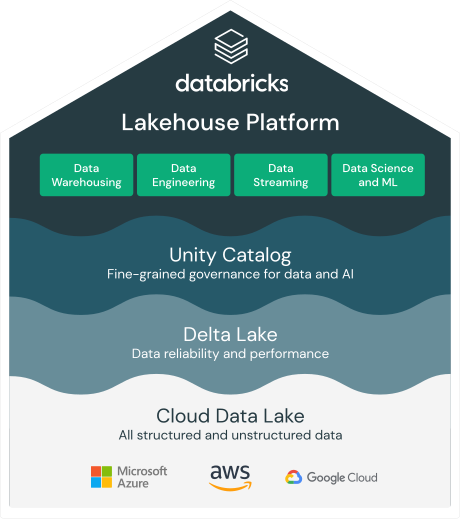
\includegraphics[width=2.4cm]{./image/Marketecture.png}
  \caption{レイクハウスプラットフォーム概略図}
  \label{lakehouse}
  \title
\end{figure}
Databricksでは新たなデータ活用プラットフォームとしてレイクハウスを提案している.
レイクハウスとはデータウェアハウスとデータレイクそれぞれの利点を組み合わせたアーキテクチャである.
データウェアハウスは画像や音声などの非構造化データの格納には適しておらず,データレイクはトランザクション・データ品質の保証等に適していないという課題があった.
データウェアハウスと同様のデータ構造とデータ管理能力を搭載している他,データレイクの低コストなストレージへの直接アクセスという特性をデータレイクは実現している.
構造化データは勿論,非構造化データ等のさまざまなデータタイプが格納できるほか,トランザクションやBI,様々な言語が同一のノートブックで使用できるなど他のプラットフォームと比較した場合大きな優位性がある.
Databricksでは新たなデータ活用プラットフォームとしてレイクハウスを提案している.
レイクハウスとはデータウェアハウスとデータレイクそれぞれの利点を組み合わせたアーキテクチャである.
データウェアハウスは画像や音声などの非構造化データの格納には適しておらず,データレイクはトランザクション・データ品質の保証等に適していないという課題があった.
データウェアハウスと同様のデータ構造とデータ管理能力を搭載している他,データレイクの低コストなストレージへの直接アクセスという特性をデータレイクは実現している.
構造化データは勿論,非構造化データ等のさまざまなデータタイプが格納できるほか,トランザクションやBI,様々な言語が同一のノートブックで使用できるなど他のプラットフォームと比較した場合大きな優位性がある.


\subsection{主要機能}
\subsubsection{Data Science \& Engineering}
Data Science \& Engineeringはデータの取得・加工を目的としたApache Sparkに基づくデータ分析プラットフォーム.
非エンジニア人材のデータ利用の促進が可能など,社内のさまざまな人材間のデータコラボレーションが可能なプラットフォームである.
Jupyter Notebook等と似ており,Databricksを初めて使用するユーザーであっても親和性の高いデザインであることが魅力的.
\begin{figure}[H]
  \centering
  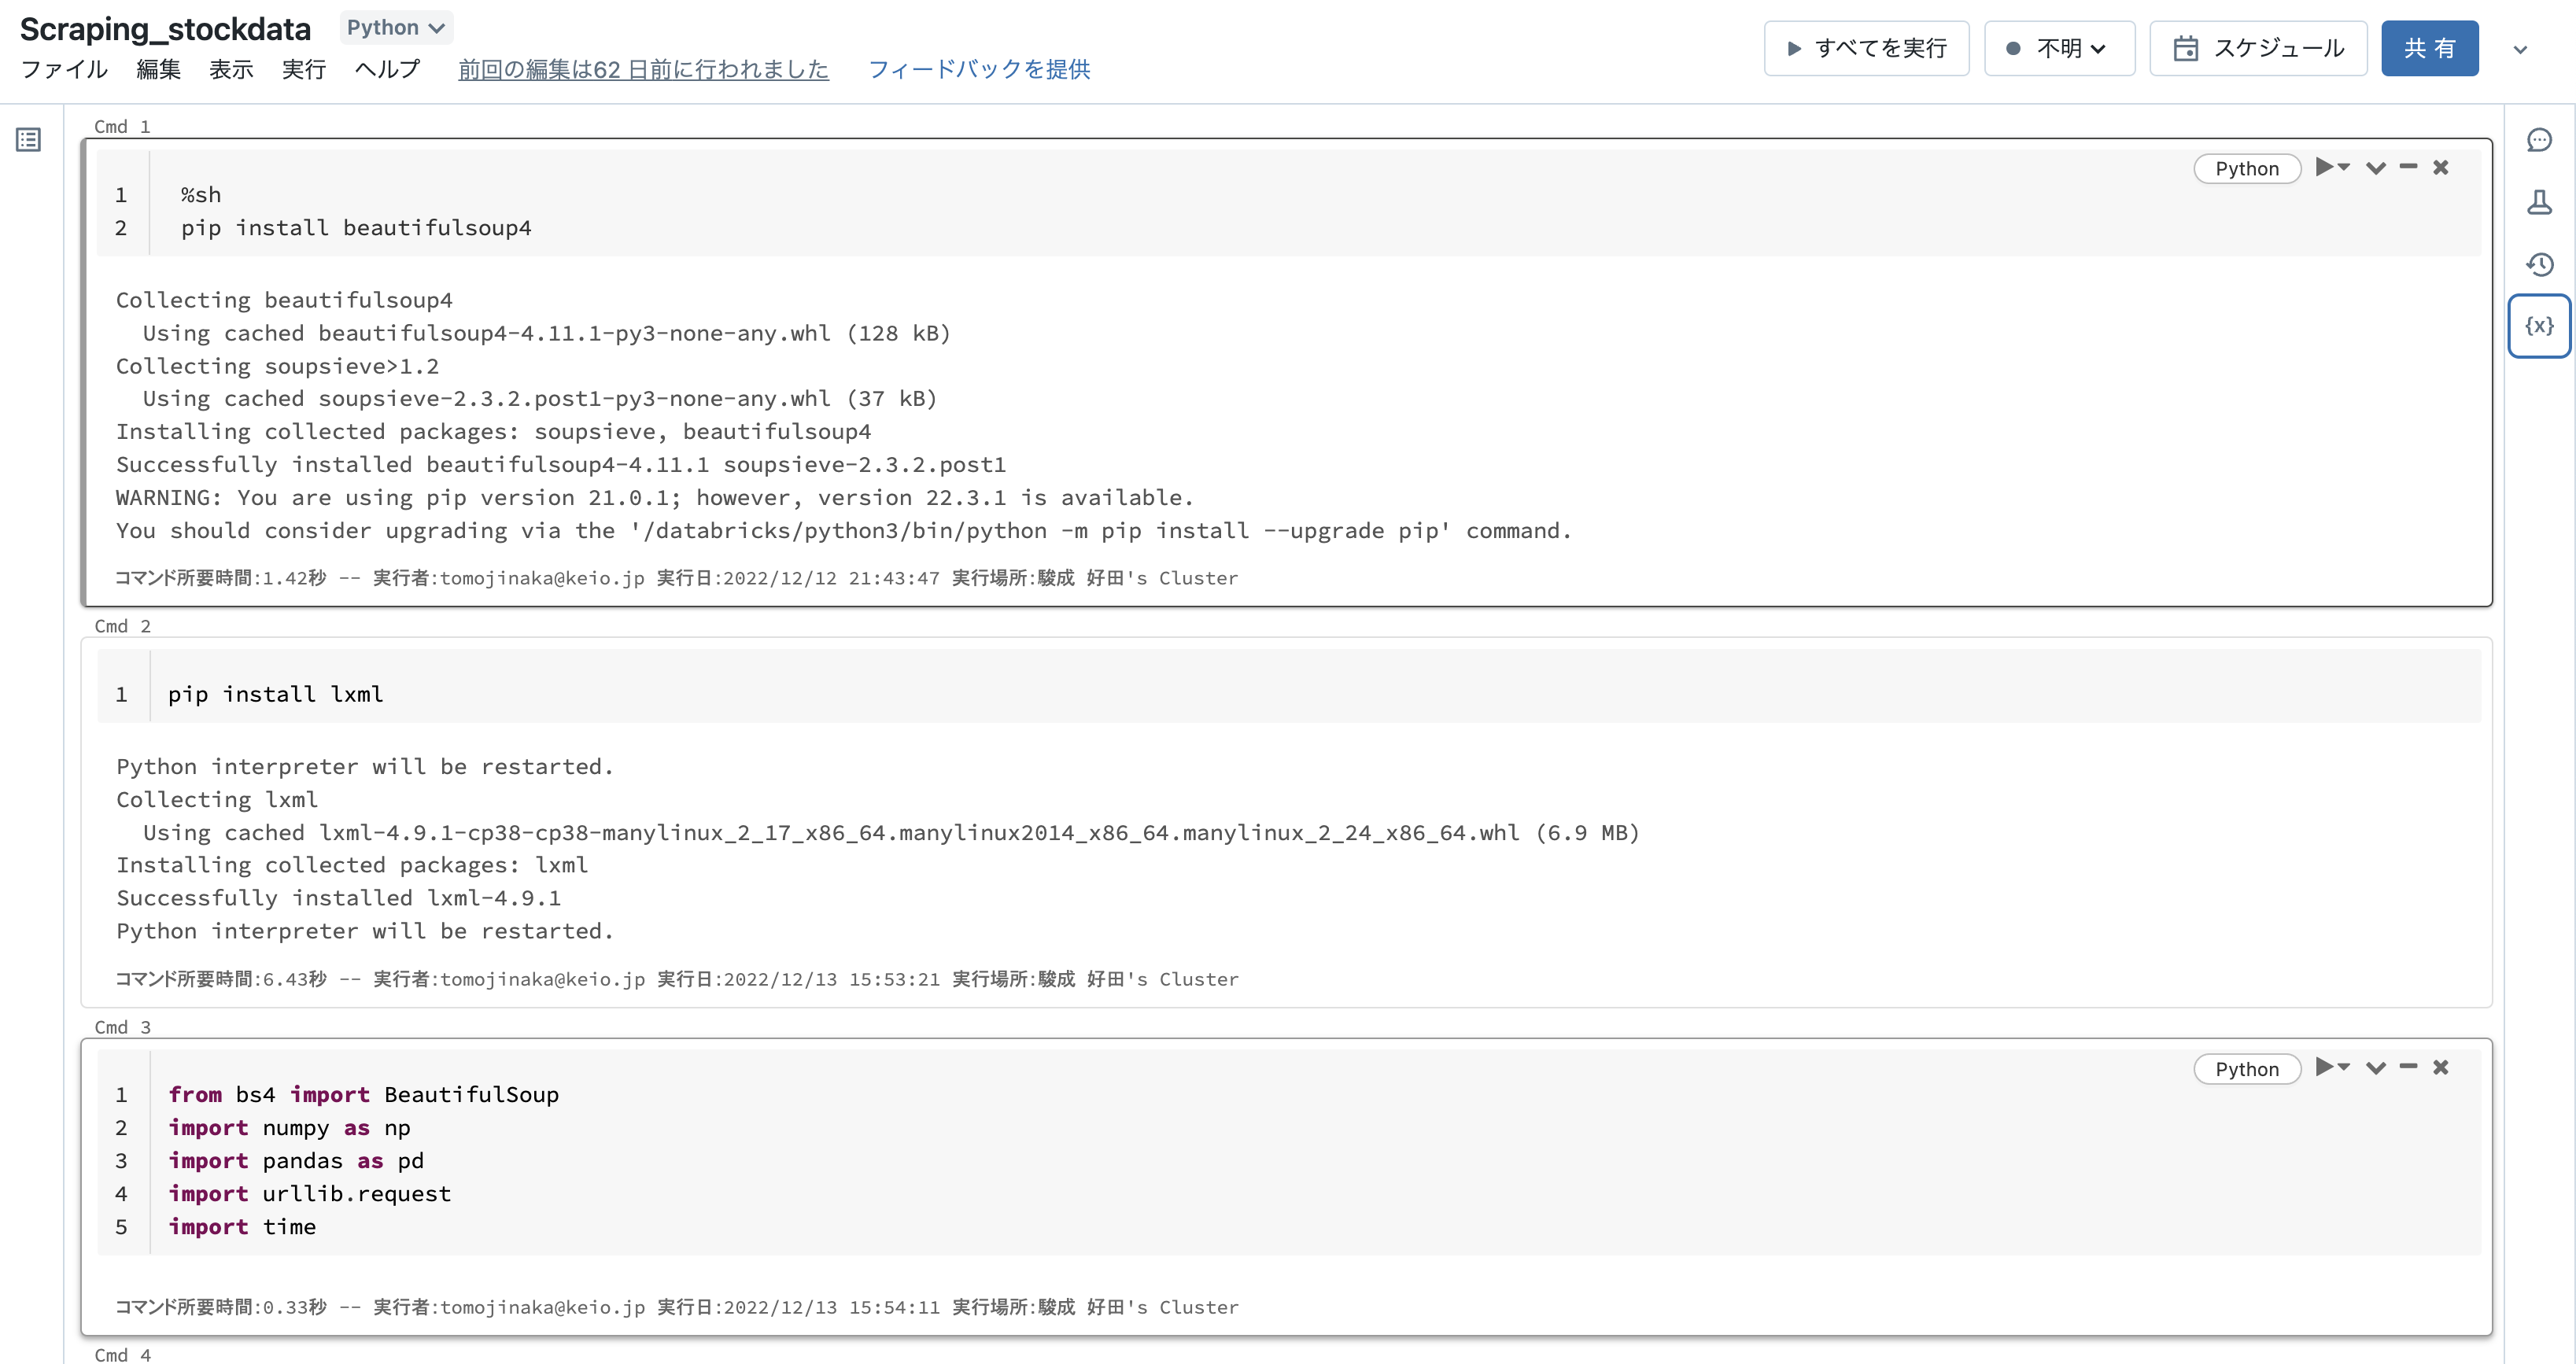
\includegraphics[height=3cm]{./image/notebook.png}
  \caption{Notebook 使用画面}
  \label{Notebook}
  \title
\end{figure}
さまざまなOSSから構成されており,特にSpark Core APIが導入されていることでR,SQL,Python,Scala,Javaを宣言一つで切り替えられる.
各ファイルはNotebookと呼ばれ,このNotebook単位でジョブを定義でき,定期実行やパイプラインの作成がGUIからも容易に設定が可能.
各ノートブックはApache Spark クラスターにより運用され,GPU・CPU性能のスケールアップ/スケールダウンが容易にでき,その設定も共有できる.
\subsubsection{Databricks SQL}
Databricks SQLは,ETL,分析,ダッシュボードの作成を行うための一連のツールが用意されているコンポーネントである.
BIツールと直結したデータウェアハウスでのダッシュボードが作成可能のため,ダッシュボード反映までのスピードが早い点が魅力.
直感的なダッシュボード構築は非エンジニア人材への配慮が多くなされている.
クラスターと同様にSQLウェアハウスと呼ばれる実行環境が用意されており,クラスター同様に必要度に応じてスケールアップ/スケールダウンを容易に実現可能である.
\begin{figure}[H]
  \centering
  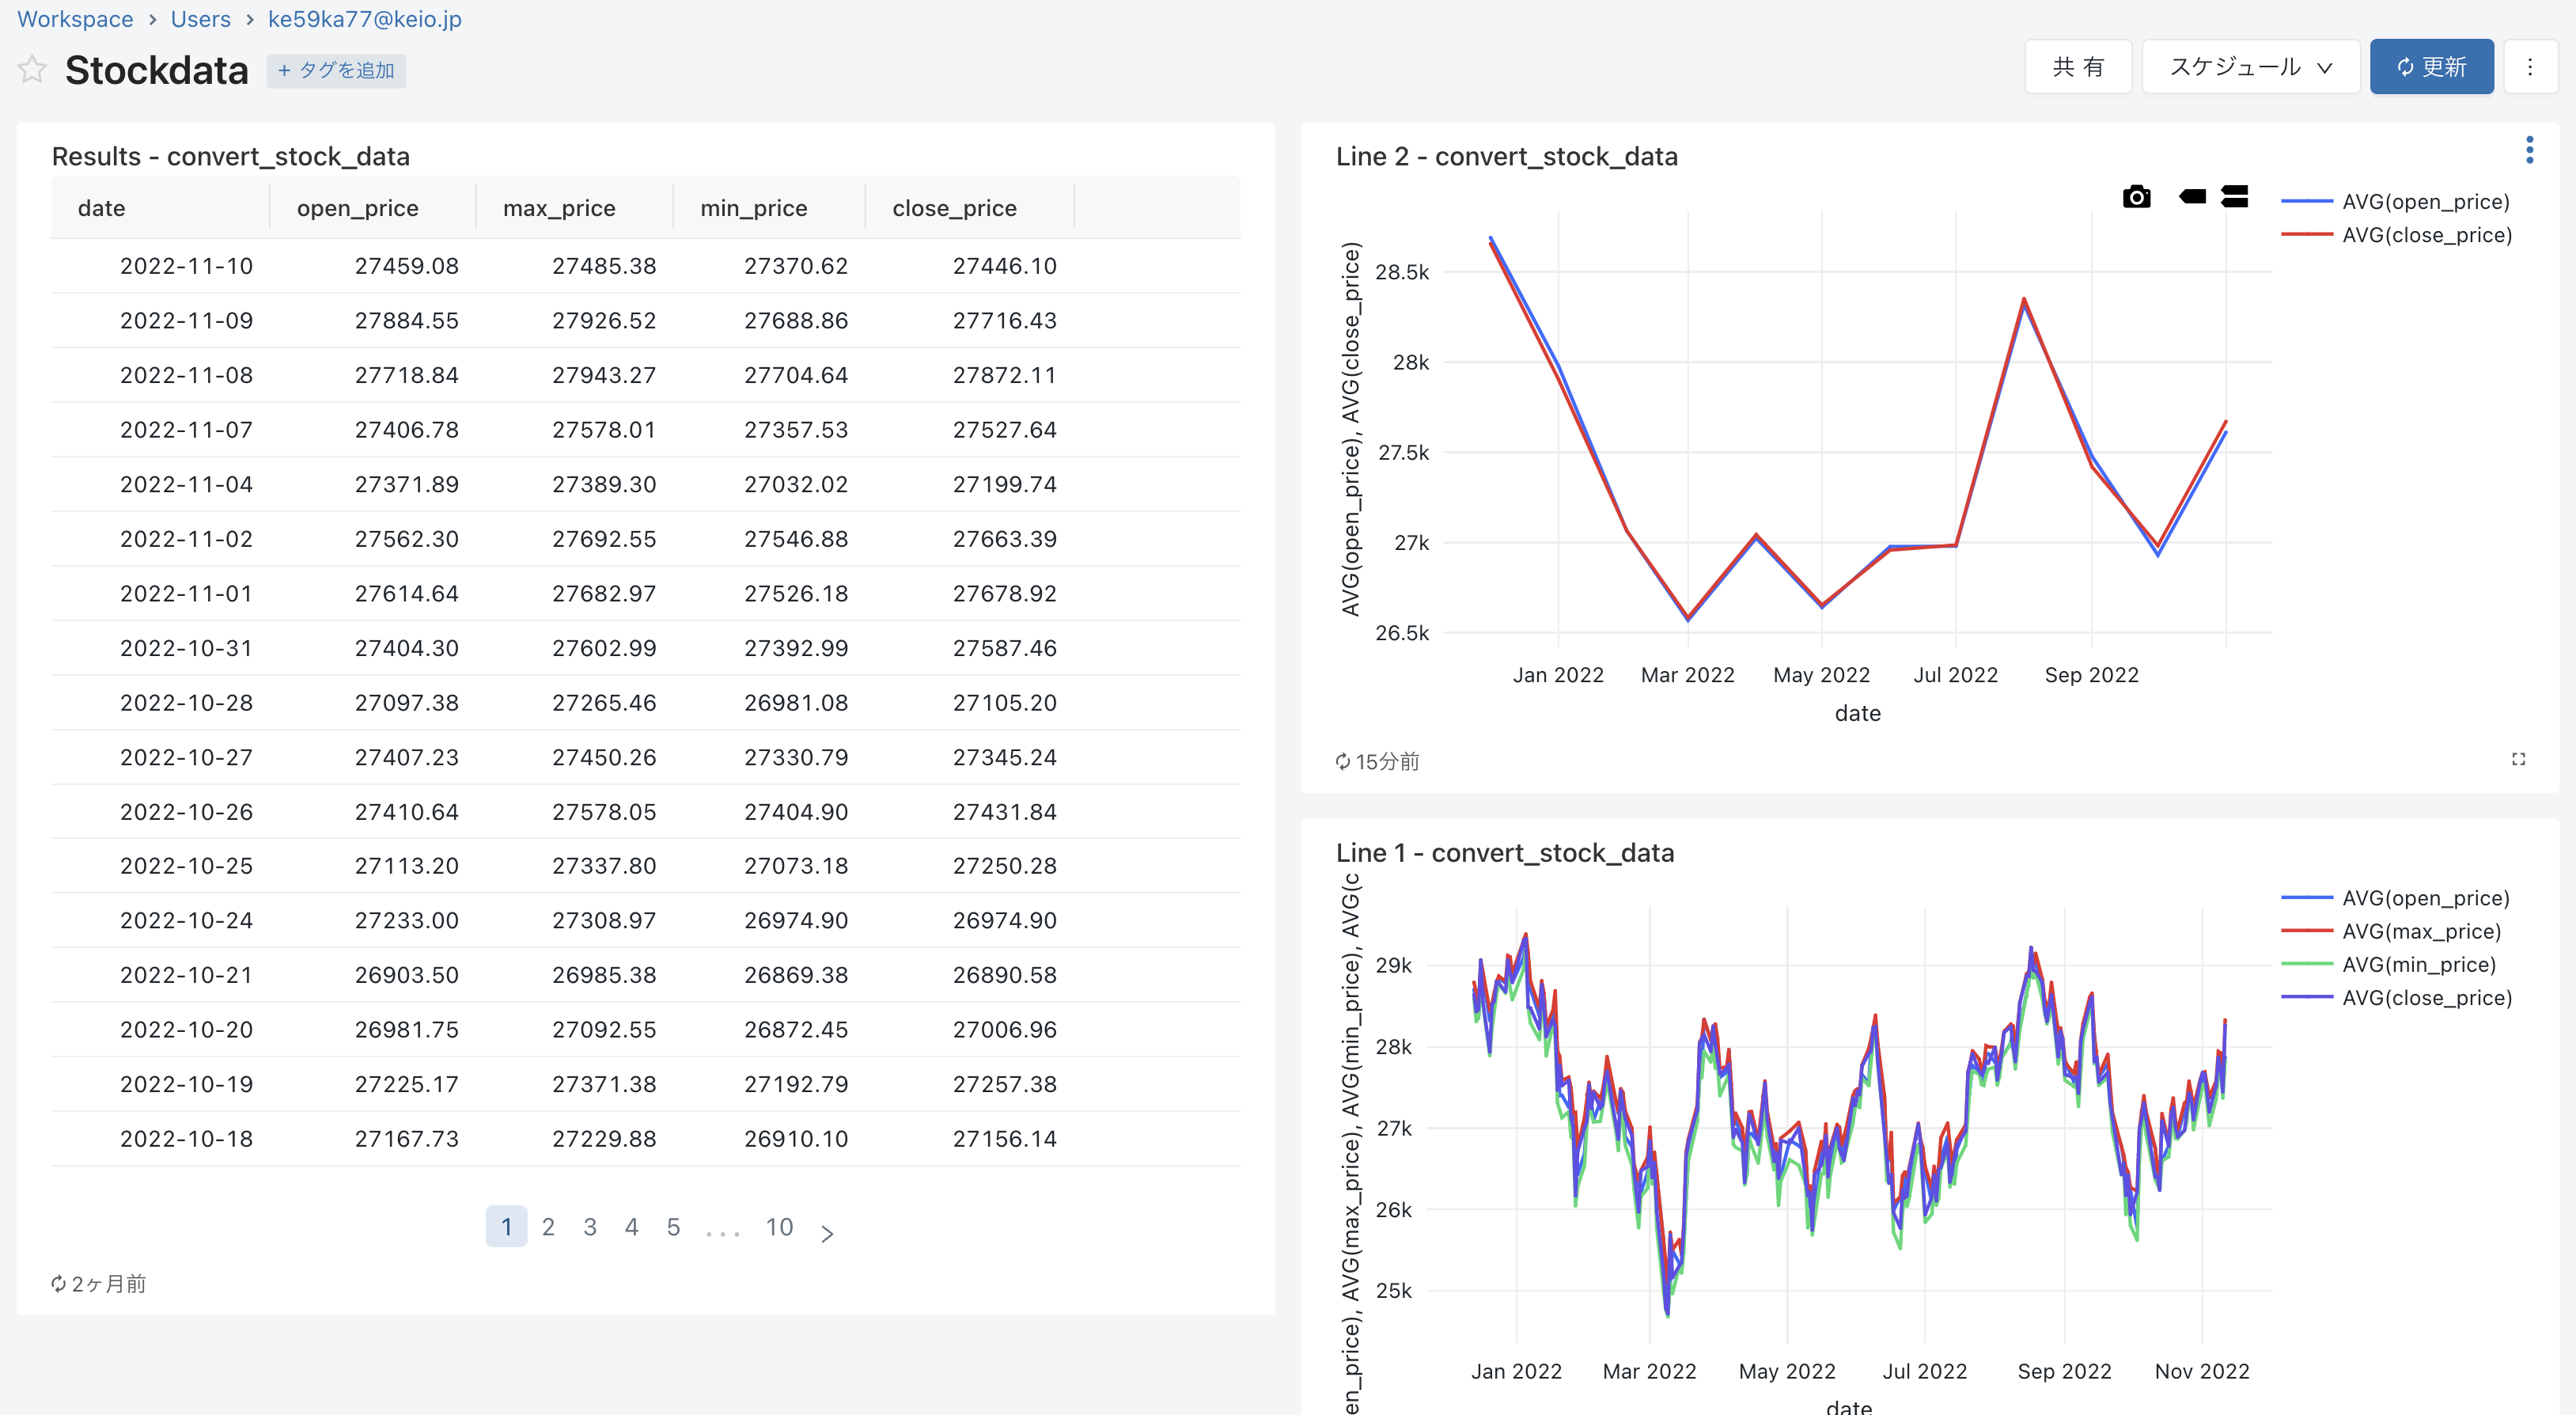
\includegraphics[height=3cm]{./image/dashboard.png}
  \caption{Databricks SQL Dashboard 使用画面}
  \label{Dashboard}
  \title
\end{figure}
\subsubsection{Databricks Machine Learning}
Databricks Machine Learningとは機械学習のモデル作成においてそのトレーニングの過程の追跡や管理を行うための機械学習プラットフォームである.
主に先述のData Science \& EngineeringのNotebookを用いてデータ加工,学習を行うおこなう.機械学習モデルの作成のため,Databricks Macine Learningでは
モデルの自動作成のためのAuto ML,ハイパーパラメーターチューニングを行うためのモデルのトレーニング状況を追跡を行うML Flowを用いた実験(Experiment)機能,モデルの共有・管理・提供のためのモデルレジストリがこのコンポーネントでは提供されており,
自前の環境では環境構築の難易度が高い機械学習向けインフラを容易に使用できるエンドツーエンドのプラットフォームである.
\section{調査結果}
\subsection{Databricksの強み}
前節までの調査をもとにDatabricksの強みをまとめる.\par
\begin{enumerate}
  \item データ活用に不可欠な環境をブラウザ上で使用できる \\
  先述の諸機能を利用してデータ収集からMLモデル運用までを一気通貫で行うことが可能
  \item コスト効率が一般に良い\\
  メンテナンス・初期導入コスト等が低く維持しやすい。
  \item クラウドインフラのリソース (コスト) 管理が容易
非エンジニアが利用することを想定したUI設計がされており,チームでの利用にとても親和性が高いプラットフォームと言える.
煩雑なクラスターの設定など低レイヤの技術が隠蔽されていることで初心者や非エンジニアにとっても利用しやく、直感的に使用可能なUIにより学習コストも削減できる.
\end{enumerate}
\subsection{大学内での使用可能性評価と今後の展開}
前述の内容より学生にとってDatabricksがオーバースペックであることは否めない.
一方で,本プロジェクトではアカデミアでDatabricksは無価値とは考えておらず、以下のような理由から有用であると考える。
第一に,学生が純粋にデータ解析のみを行いたい学生には有用なツールと言える.
Databricksには先述の通り多様なOSSによりデータ分析における様々な機能が格納されており、各種技術の学習きっかけにもなり得るツールである.
第二に,授業や研究活動においてデータ解析を手段として用いるような研究や授業で有用である.機械学習を用いて別の分野の研究を行う研究室やプロジェクトではDatabricksの活用で環境構築・維持にかかる負荷の低減が実現できる.その時間の削減により新たな発展が生まれることを期待する.
以上のような理由からDatabricksを用いたハンズオンを中心として,Git, SQL等の関連技能の講習を含めた講習会をの実施を2023年春に企画している.
\section{結論}
本プロジェクトによりDatabricksの有用性を評価することができた.ビジネス文脈で使用される機能を多く備えたツールであるという側面は理解した上で,
機械学習を使用することを目的として研究や学習用途で学生が使う有用性は大いに認められるだろう.AIC DatabricksプロジェクトとしてDatabricksの慶應義塾大学における普及・De Falcto Standard化を促進するため,Databricksに関する
授業提供を実施する.学生に機械学習が容易に活用できるという選択肢を提示することにより今後の慶應義塾大学での研究・学習における機械学習の活用が促進されることで未来の研究にポジティブに寄与してゆきたい.

\begin{thebibliography}{3}
  \tiny
  \bibitem{databricksHP} Data Lakehouse Architecture and AI Company. Databricks. (n.d.). Retrieved February 14, 2023, from https://www.databricks.com/.
  \bibitem{Gartner} Databricks、ガートナー クラウドデータベース管理システムのマジック・クアドラントのリーダーの 1 社に. Databricks. (n.d.). Retrieved February 15, 2023, from https://www.databricks.com/jp/resources/analyst-paper/databricks-named-leader-by-gartner
  \bibitem{about_databricks} Mssaperla. (n.d.). Azure Databricks のドキュメント. Microsoft Learn. Retrieved February 15, 2023, from https://learn.microsoft.com/ja-jp/azure/databricks/ 
  \end{thebibliography}
\end{document}
%\label{lakehouse} $\url{https://www.databricks.com/jp/product/data-lakehouse}$]
